\newpage
\clearpage
\appendix
\appendixpage

\section{Implementation Details}
\paragraph{Optimization Objective.} 
In addition to the typical MSE Loss~\cite{ho2020denoising} used in the Latent Diffusion Model (LDM), we also incorporate StyleCLIP~\cite{patashnik2021styleclip} loss to guide the model toward the correct manipulation direction.  Formally,

\begin{equation}
\begin{aligned}
    \mathcal{L}_{style} &= 1 - \\
    \mathcal{D}(
    \textbf{F}_{vis}(\hat{Y}^{edit}) &- \textbf{F}_{vis}(Y), 
    \textbf{F}_{text}(T^{edit}) - \textbf{F}_{text}(T)),
\end{aligned}
\end{equation}

where $\mathcal{D}$ indicates the cosine similarity between two vectors. 
$Y$ and $T$ represent the original visual stimuli and its corresponding text, while the $\hat{Y}^{edit}$ and $T^{edit}$ are the synthesized result produced by our network and its corresponding ground truth caption, respectively. $\hat{Y}^{edit}$ can be estimated at each time step as follows:
\begin{equation}
\label{eq:decode_z}
    \hat{\textbf{z}}_0^e = (\textbf{z}_t^e - \sqrt{1-\overline{\alpha}_t} \bm{\epsilon}_{\theta} (\textbf{z}_t^e)) / \sqrt{\overline{\alpha}}_t,
\end{equation}
where the $\overline{\alpha}_t := \prod_{s=1}^t \alpha_s$. 
$\hat{Y}^{edit}$ can be decoded from $\hat{\textbf{z}}_0^e$.
The functions $\textbf{F}_{vis}$ and $\textbf{F}_{text}$ represent the CLIP backbone used to extract the visual and text features, respectively.
Such formulation ensures that the editing direction of the synthesized image aligns closely with the text direction in CLIP space.
The overall loss function, which combines the style direction loss with the foundational LDM loss, is mathematically represented as:
\begin{equation}
\mathcal{L}=\mathcal{L}_{simple}+\sqrt{\bar{\alpha}_t} \mathcal{L}_{style},
\end{equation}
where $\sqrt{\bar{\alpha}_t}$ is leveraged to emphasize the supervision with lower noise input (i.e., smaller time-step) and reduce the impact with higher noise (i.e., larger time-step).



\paragraph{Inference Paradigm.} Given a target fMRI signal $X$, our goal is to interact with it through the instruction $I$. The primary objective is to manipulate the visual content within the human brain toward the desired direction, resulting in $Y^{edit}$. During inference, we first use $\bm{g}_\theta(\textbf{z}^r_t, X, t)$ to perform $K$ diffusion steps for basic feature formation from $X$. Building on this, the dual-stream diffusion model $\bm{\epsilon}_\theta(\textbf{z}^r_t, \textbf{z}^e_t, I, X, t)$ progressively guides the fMRI signal.
After the diffusion process is complete, the latent code $\textbf{z}_0^e$ is transformed back to $Y^{edit}$ following Equation~\ref{eq:decode_z}. The detailed inference process is depicted in Algorithm~\ref{alg:test}.

\begin{algorithm*}[!ht]
  \caption{Inference of the asynchronous dual-stream diffusion model $\bm{\epsilon}_{\theta}$}
  \label{alg:sampling}
  \label{alg:test}
  \small
  \begin{algorithmic}[1]
    \vspace{.04in}
    \State $  \textbf{z}_T^e \sim \mathcal{N}(\mathbf{0}, \mathbf{I}), $ $  \textbf{z}_T^r \sim \mathcal{N}(\mathbf{0}, \mathbf{I})  $

    \For{$t=T, \dotsc, T-K+1$}
      \State $\textbf{z}^{nr} \sim \mathcal{N}(\mathbf{0}, \mathbf{I})$
      \State $\textbf{z}^r_{t-1} = \frac{1}{\sqrt{\alpha_t}}\left( \textbf{z}^r_{t} - \frac{1-\alpha_t}{\sqrt{1-\bar{\alpha}_t}} \bm{g}_\theta(\textbf{z}^r_{t}, X,t) \right) + \sigma_t \textbf{z}^{nr}$
    \EndFor

    \For{$t=T, \dotsc, K+1$}
      \State $\textbf{z}^{nr} \sim \mathcal{N}(\mathbf{0}, \mathbf{I})$ if $t > K+1$, else $\textbf{z}^{nr} = \mathbf{0}$
      \State $\textbf{z}^{ne} \sim \mathcal{N}(\mathbf{0}, \mathbf{I})$
      \State $\textbf{z}^r_{t\textcolor{red}{-K}-1} = \frac{1}{\sqrt{\alpha_{t\textcolor{red}{-K}}}}\left( \textbf{z}^r_{t\textcolor{red}{-K}} - \frac{1-\alpha_{t\textcolor{red}{-K}}}{\sqrt{1-\bar{\alpha}_{t\textcolor{red}{-K}}}} \bm{g}_\theta(\textbf{z}^r_{t\textcolor{red}{-K}}, X,t\textcolor{red}{-K}) \right) + \sigma_{t\textcolor{red}{-K}} \textbf{z}^{nr}$
      \State $\textbf{z}^e_{t-1} = \frac{1}{\sqrt{\alpha_t}}\left( \textbf{z}^e_{t} - \frac{1-\alpha_t}{\sqrt{1-\bar{\alpha}_t}} \bm{\epsilon}_\theta(\textbf{z}^r_{t\textcolor{red}{-K}}, \textbf{z}^e_{t}, I,X,t) \right) + \sigma_t \textbf{z}^{ne}$
    \EndFor

    \For{$t=K, \dotsc, 1$}
      \State $\textbf{z}^{ne} \sim \mathcal{N}(\mathbf{0}, \mathbf{I})$ if $t > 1$, else $\textbf{z}^{ne} = \mathbf{0}$
      \State $\textbf{z}^e_{t-1} = \frac{1}{\sqrt{\alpha_t}}\left( \textbf{z}^e_{t} - \frac{1-\alpha_t}{\sqrt{1-\bar{\alpha}_t}} \bm{\epsilon}_\theta(\textbf{z}^r_0, \textbf{z}^e_{t}, I,X,t) \right) + \sigma_t \textbf{z}^{ne}$

    \EndFor
    
    \State \textbf{return} $\textbf{z}^e_0$
    \vspace{.04in}
  \end{algorithmic}
\end{algorithm*}

\paragraph{Training Paradigm.}
During training, the denoising operation is performed asynchronously, with the instruction flow lagging behind by $K$ time steps. The detailed training process of our dual-stream diffusion framework is outlined in Algorithm~\ref{alg:training}.

\begin{algorithm*}[h]
  \caption{Training of the asynchronous dual-stream diffusion model $\bm{\epsilon}_{\theta}$}
  \label{alg:training}
  \small
  \begin{algorithmic}[1]
    \Repeat
      \State $(\textbf{z}_0^e, \textbf{z}_0^r, I, X) \sim q(\textbf{z}_0^e, \textbf{z}_0^r, I, X)$
      \State $\bm{\epsilon} \sim \mathcal{N}(\mathbf{0}, \mathbf{I}), \bm{\epsilon}^r \sim \mathcal{N}(\mathbf{0}, \mathbf{I})$
      \State $t \sim \text{Uniform}({K+1,\ldots,T})$
      \State Take a gradient descent step on
      \State 
      $ \quad \nabla_\theta \left\| \bm{\epsilon} - \bm{\epsilon}_\theta(\sqrt{\bar{\alpha}_{t\textcolor{red}{-K}}} \textbf{z}_0^r+\sqrt{1-\bar{\alpha}_{t\textcolor{red}{-K}}} \bm{\epsilon}^r, 
      \sqrt{\bar{\alpha}_{t}} \textbf{z}_0^e+\sqrt{1-\bar{\alpha}_{t}} \bm{\epsilon}, I, X, t) \right\|$
    \Until{converged}
  \end{algorithmic}
\end{algorithm*}


\section{More Ablation Studies}
In this section, we provide a detailed quantitative analysis of the components involved in our method.
Firstly, we present both qualitative and quantitative results to illustrate the impact of varying asynchronous steps.
Next, we offer further insights into the design of the dual-stream architecture.
Finally, we include additional qualitative ablation results to demonstrate the effect of each part of our architecture.

\paragraph{Impact of Varied Asynchronous Steps.} To investigate the impact of delayed steps on model performance, we conduct experiments with varied time steps. Specifically, in our implementation, we adopt $T=50$ at inference for efficiency. Thus, we choose $K=0, 5, 15, 25, 35$, which are broadly distributed, to conduct the experiment. For the sake of comparison, we do not incorporate LLMs and manually fix the random seed for all settings. Table~\ref{table:ablate_time_steps} illustrates the impact of delayed time steps. We observe that overall performance improves as we increase the delayed time steps, but the improvement becomes marginal beyond $K=15$. This is likely because $K=15$ is sufficient for basic feature formation.


% Table 2%%%%%%%%%%%%%%%%%%%%%%%%%%%%%%%%%%%%%%%%%%%%%%%%%%%%%%%%%%%%
\begin{table*}[h] %\footnotesize
\setlength{\tabcolsep}{28pt}
\begin{center}  
\caption{\textbf{The impact of different delayed time steps on model performance.}}
% \vspace{-2pt}
\label{table:ablate_time_steps}
\begin{tabular}{lcccccccc}
\toprule
 % & \multicolumn{4}{c}{Low-Level}& \multicolumn{4}{c}{High-Level} \\
% \cmidrule(lr){2-5} \cmidrule(lr){6-9}
Delay Steps & 0 & 5 &  15 & 25 &
35 \\

\midrule  
\textbf{CLIP-I} & 0.636 & 0.638 & \textbf{0.642} & 0.642 & 0.641  \\
\textbf{Dino-I} & \textbf{0.307} & 0.307 & 0.295 & 0.295 & 0.293 \\
\textbf{CLIP-D} & 0.108 & 0.109 & \textbf{0.114} & 0.106 & 0.108 \\
% \hline
% \textbf{Mind-Sculpting}  & \textbf{0.327} & 0.315 & \textbf{0.951} & \textbf{0.978} & \textbf{0.939} \\
\bottomrule
\end{tabular}
\end{center}
% \vspace{-12pt}
\end{table*}
% Table 2%%%%%%%%%%%%%%%%%%%%%%%%%%%%%%%%%%%%%%%%%%%%%%%%%%%%%%%%%%%%



To further demonstrate the effect of the asynchronous strategy, we present the intermediate manipulation process in Fig.\ref{fig:async_demo}. We compare the synchronous strategy (set $K=0$ in the second row) with the asynchronous strategy (set $K=15$ in the third row). The individual intends to "Make it a unicorn" to manipulate brain activity. In the synchronous scenario, the model fails to capture the pertinent structure, i.e., the horse, for effective instruction (as indicated by the color of the horse within the red box). Without allowing basic feature formation in advance, the instruction model encounters difficulty in identifying the relevant structure. For additional visual results, readers can refer to Fig.\ref{fig:async_all_supp}.



\begin{figure*}[ht!]
  \centering
  % \vspace{-10pt}
  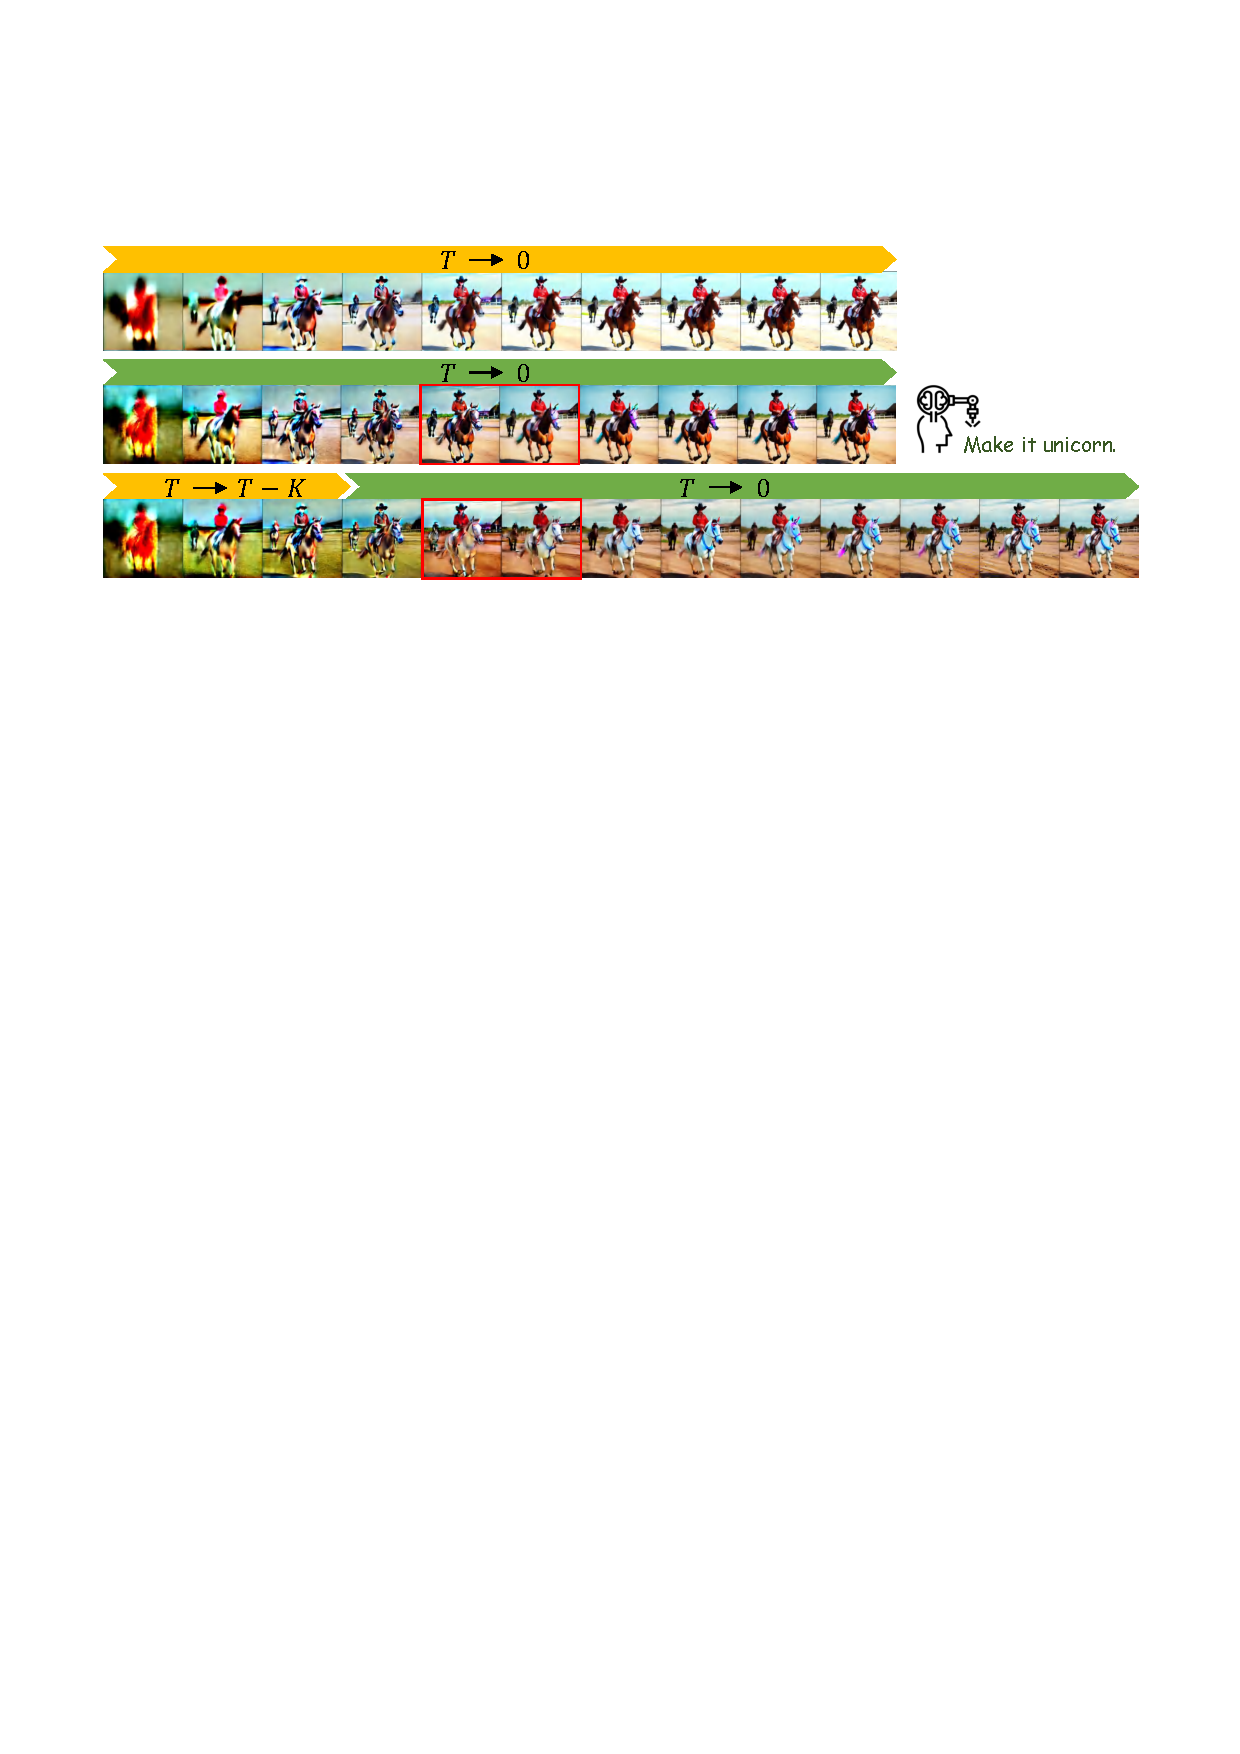
\includegraphics[width=1.0\linewidth]{figs/async_demo.pdf}
  \caption{The first row displays the intermediate reconstruction results, while the second and third rows showcase the instruction performance using synchronous and asynchronous paradigms, respectively. The orange progress bar indicates the reconstruction timeline, while the green progress bar represents the instruction timeline.}
  \label{fig:async_demo}
\end{figure*}


\begin{figure*}[ht!]
  \centering
  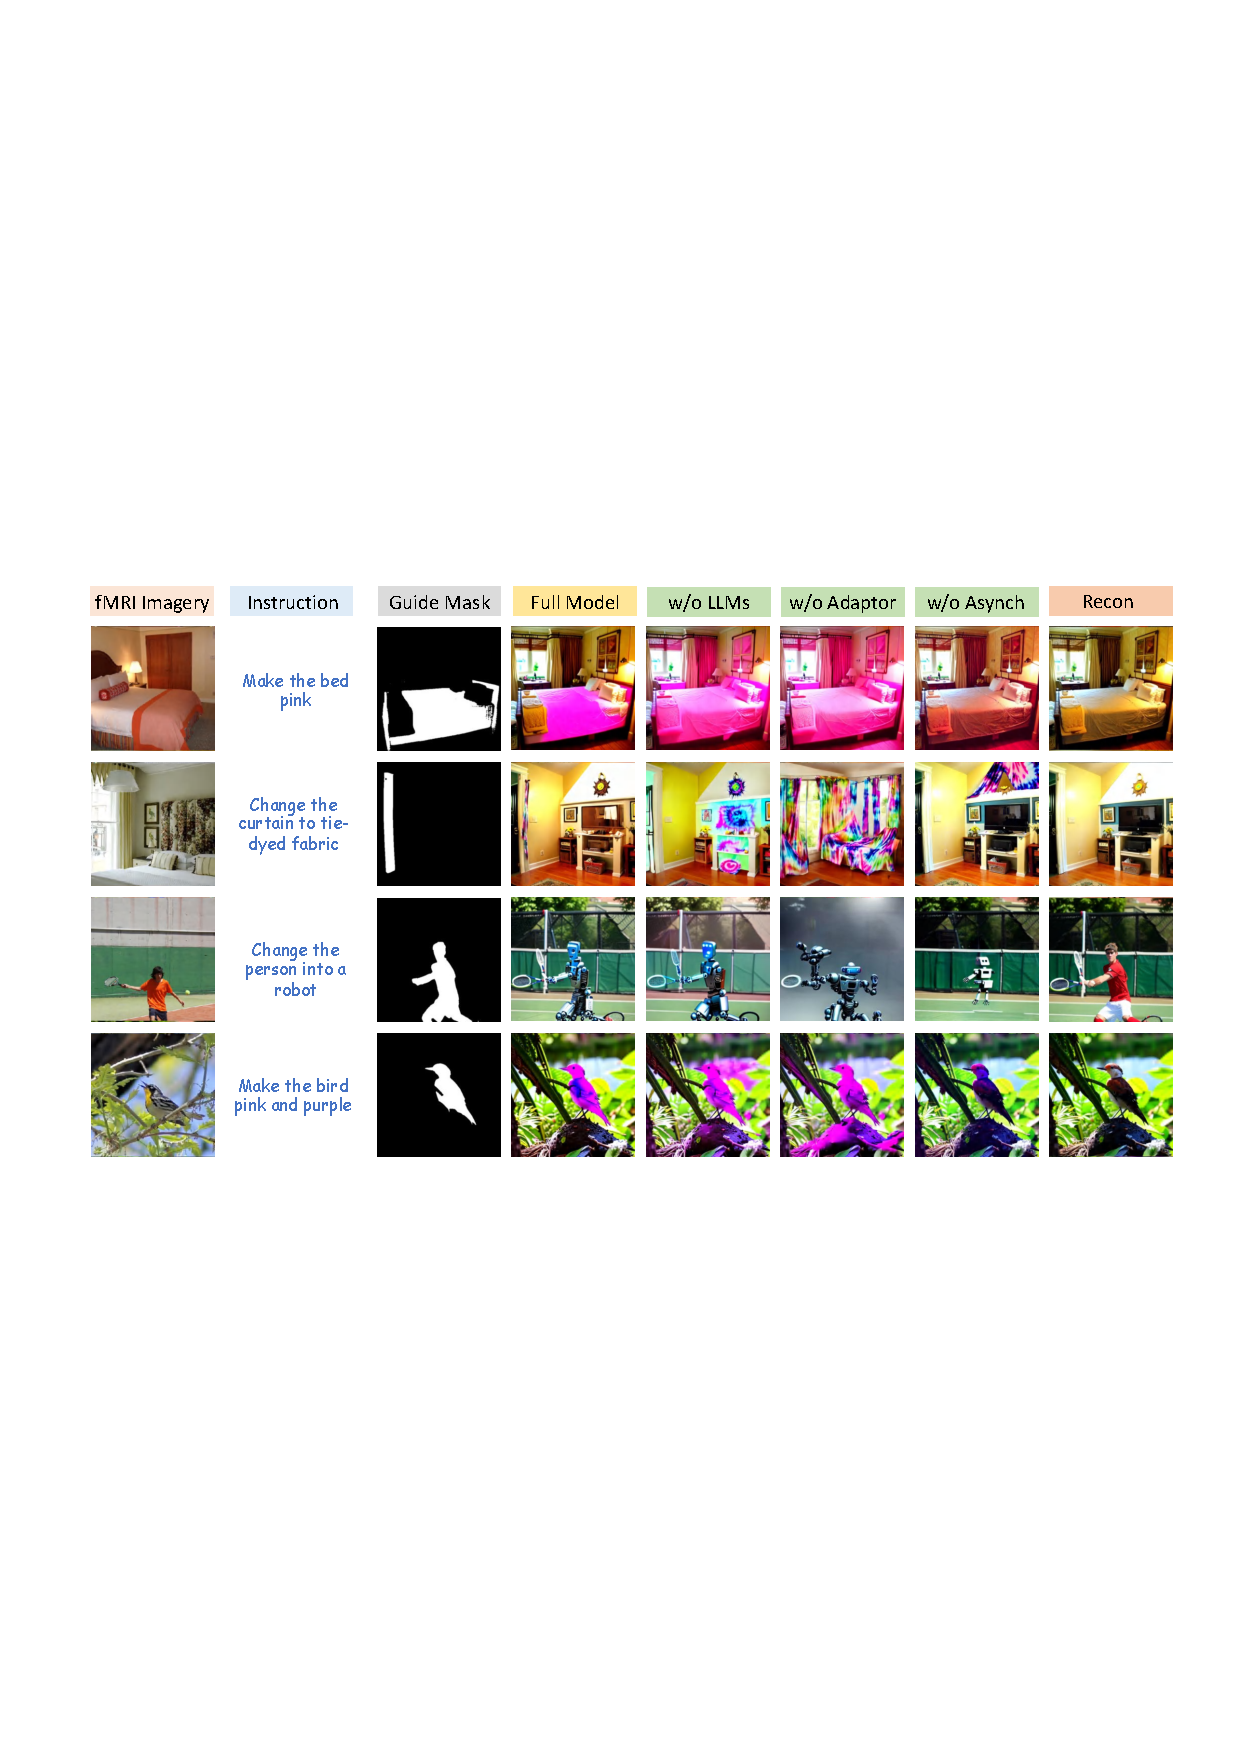
\includegraphics[width=1.0\textwidth]{figs/more_ablations.pdf} 
    % \vspace{-4pt}
  \caption{Without feature injection from adaptor, the model struggles on balancing content preservation and instruction conformation. Removing asynchronous strategy brings difficulty on instruction conformation. Through the incorporation of LLMs guided region, our framework is able to precisely operate on relevant spatial locations.}
  \label{fig:more_ablation}
  % \vspace{-5pt}
\end{figure*}


\paragraph{Impact of Injection Strategy.} The feature injection module acts as a connector, linking the instruction flow to the generation flow, ensuring seamless progressive bridging and effective instruction delivery. For the architecture design of our injection module, we explored both convolution-based structures~\cite{zhang2023adding} and transformer-based structures~\cite{hu2023animate}. Experiments demonstrate that the transformer-based architecture does not improve performance. We speculate this is because the convolution operation's advantage in maintaining spatial layout facilitates learning. Regarding the injection strategy, we empirically found that injection through ResBlock outperforms other blocks. Additionally, leveraging more advanced fusion techniques, such as transformers, does not enhance our performance.

\paragraph{More Qualitative Results.} We demonstrate additional visual results of our ablation study in Fig.~\ref{fig:more_ablation}. Eliminating the asynchronous strategy makes it difficult for the instruction flow to comprehend the aligned visual content, leading to inferior performance (see the bed and robot). Without the feature injection from the adaptor, the instruction flow lacks sufficient visual information to identify instruction-relevant regions (see the mis-edited curtain and bird). Without LLMs, the model struggles to perform precise operations within the intended spatial regions (see the bed and the bird). The full model effectively balances identity preservation and instruction conformation, achieving visually pleasing results.

\section{More fMRI Instruction Results}
In this section, we present additional visual instruction results. Although our approach is designed for language-guided instruction, it can readily extend to visual instruction with minimal effort.

\paragraph{Natural Language Instruction.}
We demonstrate more instruction results in Fig.~\ref{fig:supp_edit0} and Fig.~\ref{fig:supp_edit1}.
It can be seen that our approach is able to effectively interface with brain activity conforming to human instructions.

\paragraph{Style Manipulation.}
For style manipulation, we first invert the style reference image to a word embedding ${[V]}$ in the text latent space, following the common inversion strategy~\cite{ruiz2023dreambooth,mokady2023null}. We then use \emph{In the style of} $[V]$ as our new instruction. The results of this instruction are depicted in Fig.~\ref{fig:supp_style}. It can be seen that our approach effectively captures the style of the reference image and applies it to the target.


\begin{figure*}[ht!]
  \centering
  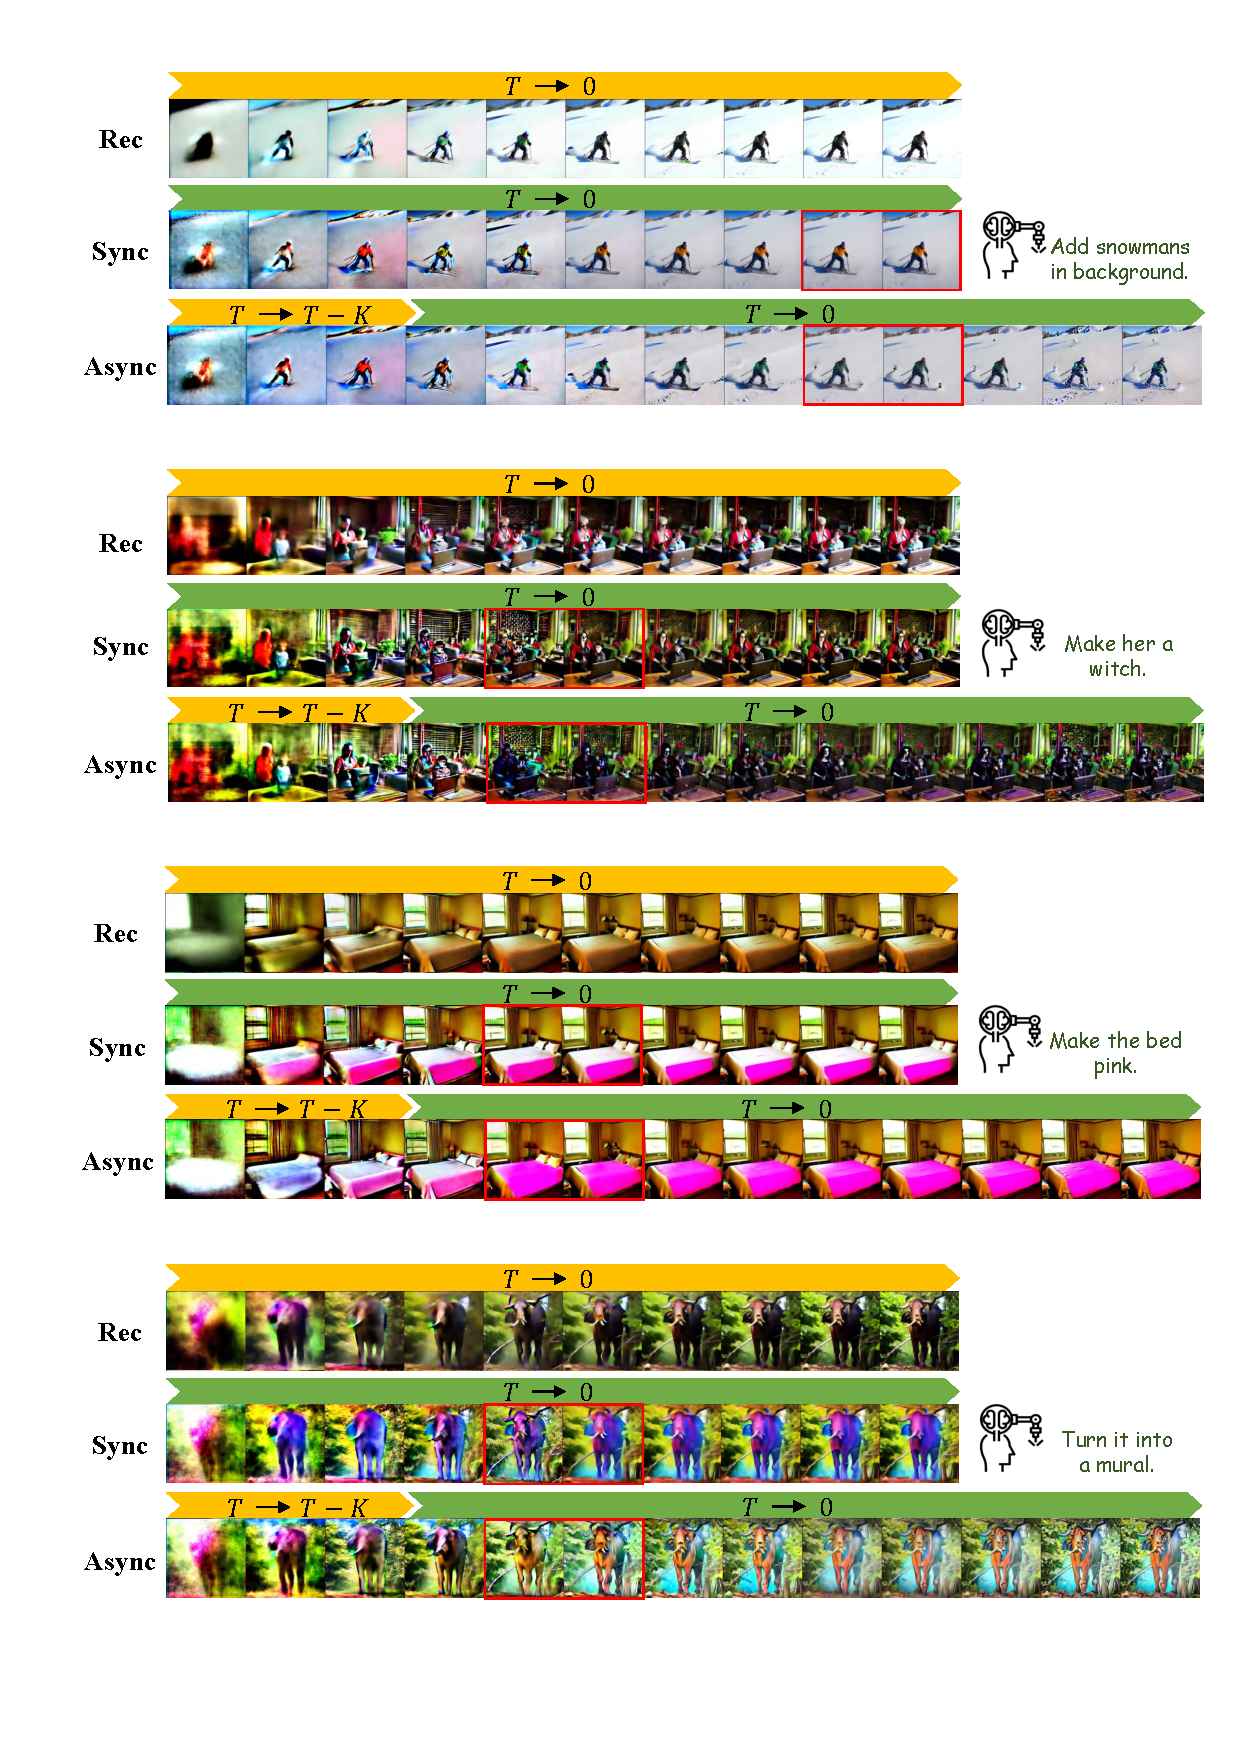
\includegraphics[width=1.0\textwidth]{figs/async_all_supp.pdf} 
    % \vspace{-4pt}
  \caption{The first row displays the intermediate reconstruction results, while the second and third rows showcase the instruction performance using synchronous and asynchronous paradigms, respectively. The orange progress bar indicates the reconstruction timeline, while the green progress bar represents the instruction timeline.}
  \label{fig:async_all_supp}
  % \vspace{30pt}
\end{figure*}



\begin{figure*}[ht!]
  \centering
  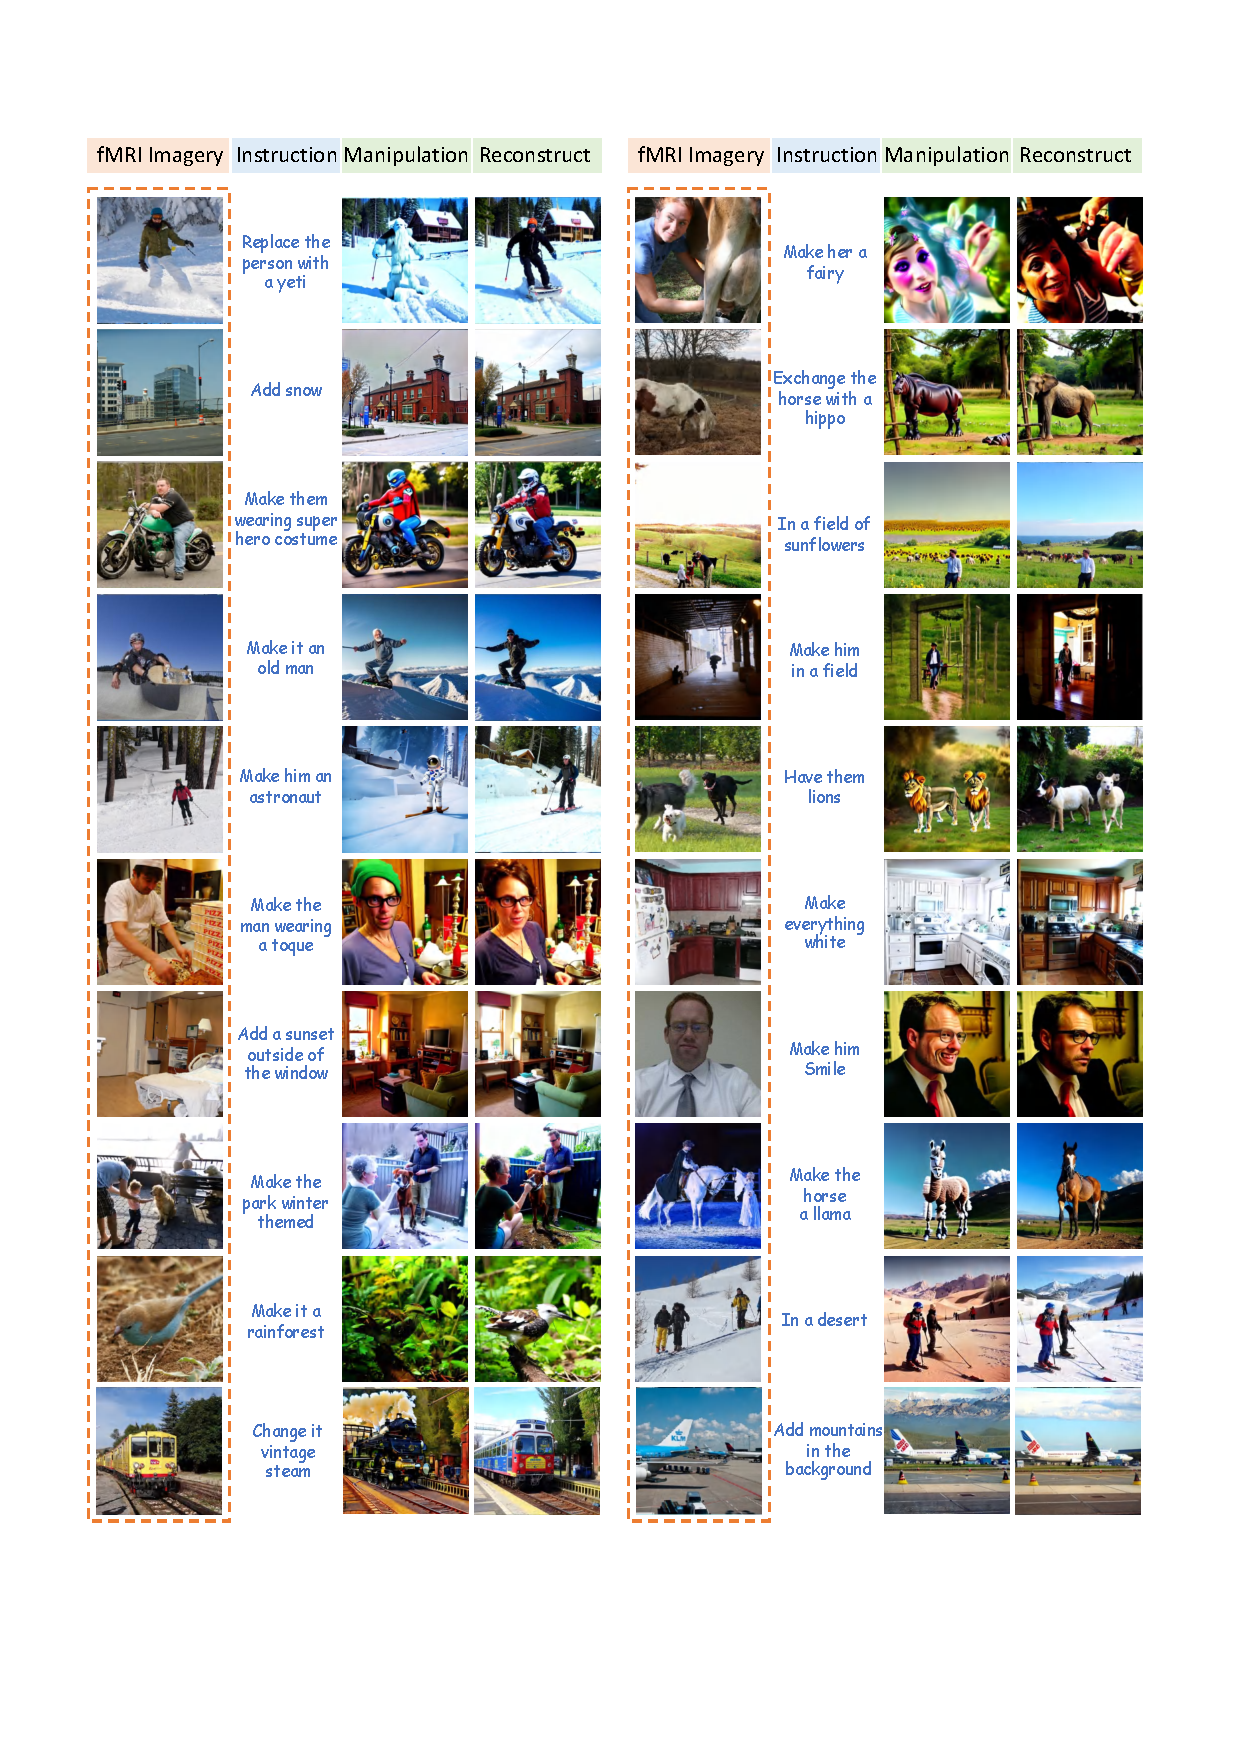
\includegraphics[width=1.0\textwidth]{figs/supp_edit0.pdf} 
    % \vspace{-4pt}
  \caption{\textbf{fMRI signal instruction with natural language description.} The first column displays the brain's visual stimulus. The second column illustrates the individual's intended operation. The third column presents the instruction results, while the fourth column shows the intermediate reconstruction results generated by our model.}
  \label{fig:supp_edit0}
  % \vspace{20pt}
\end{figure*}

\begin{figure*}[ht!]
  \centering
  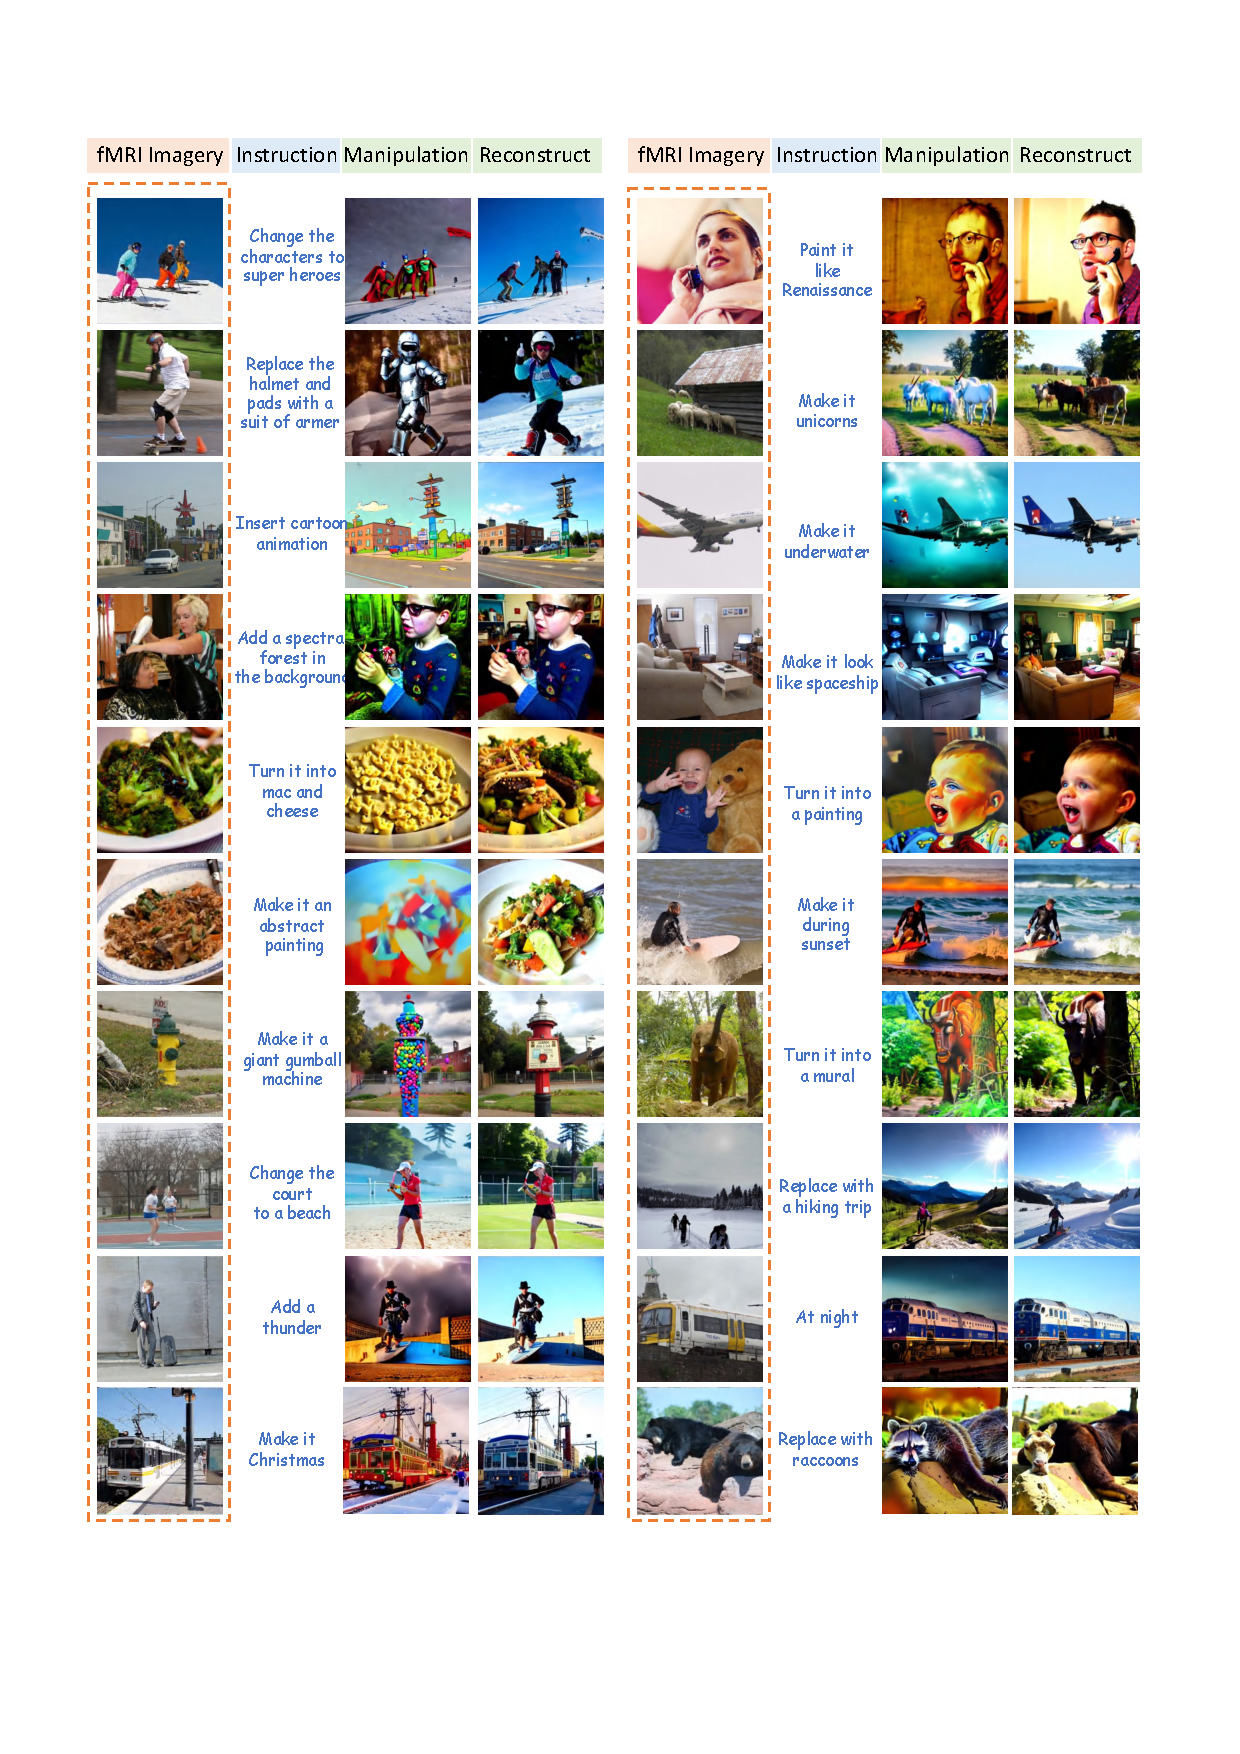
\includegraphics[width=1.0\textwidth]{figs/supp_edit1.pdf} 
    % \vspace{-4pt}
  \caption{\textbf{fMRI signal instruction with natural language description.} The first column displays the brain's visual stimulus. The second column illustrates the individual's intended operation. The third column presents the instruction results, while the fourth column shows the intermediate reconstruction results generated by our model.}
  \label{fig:supp_edit1}
  % \vspace{30pt}
\end{figure*}


\begin{figure*}[ht!]
  \centering
  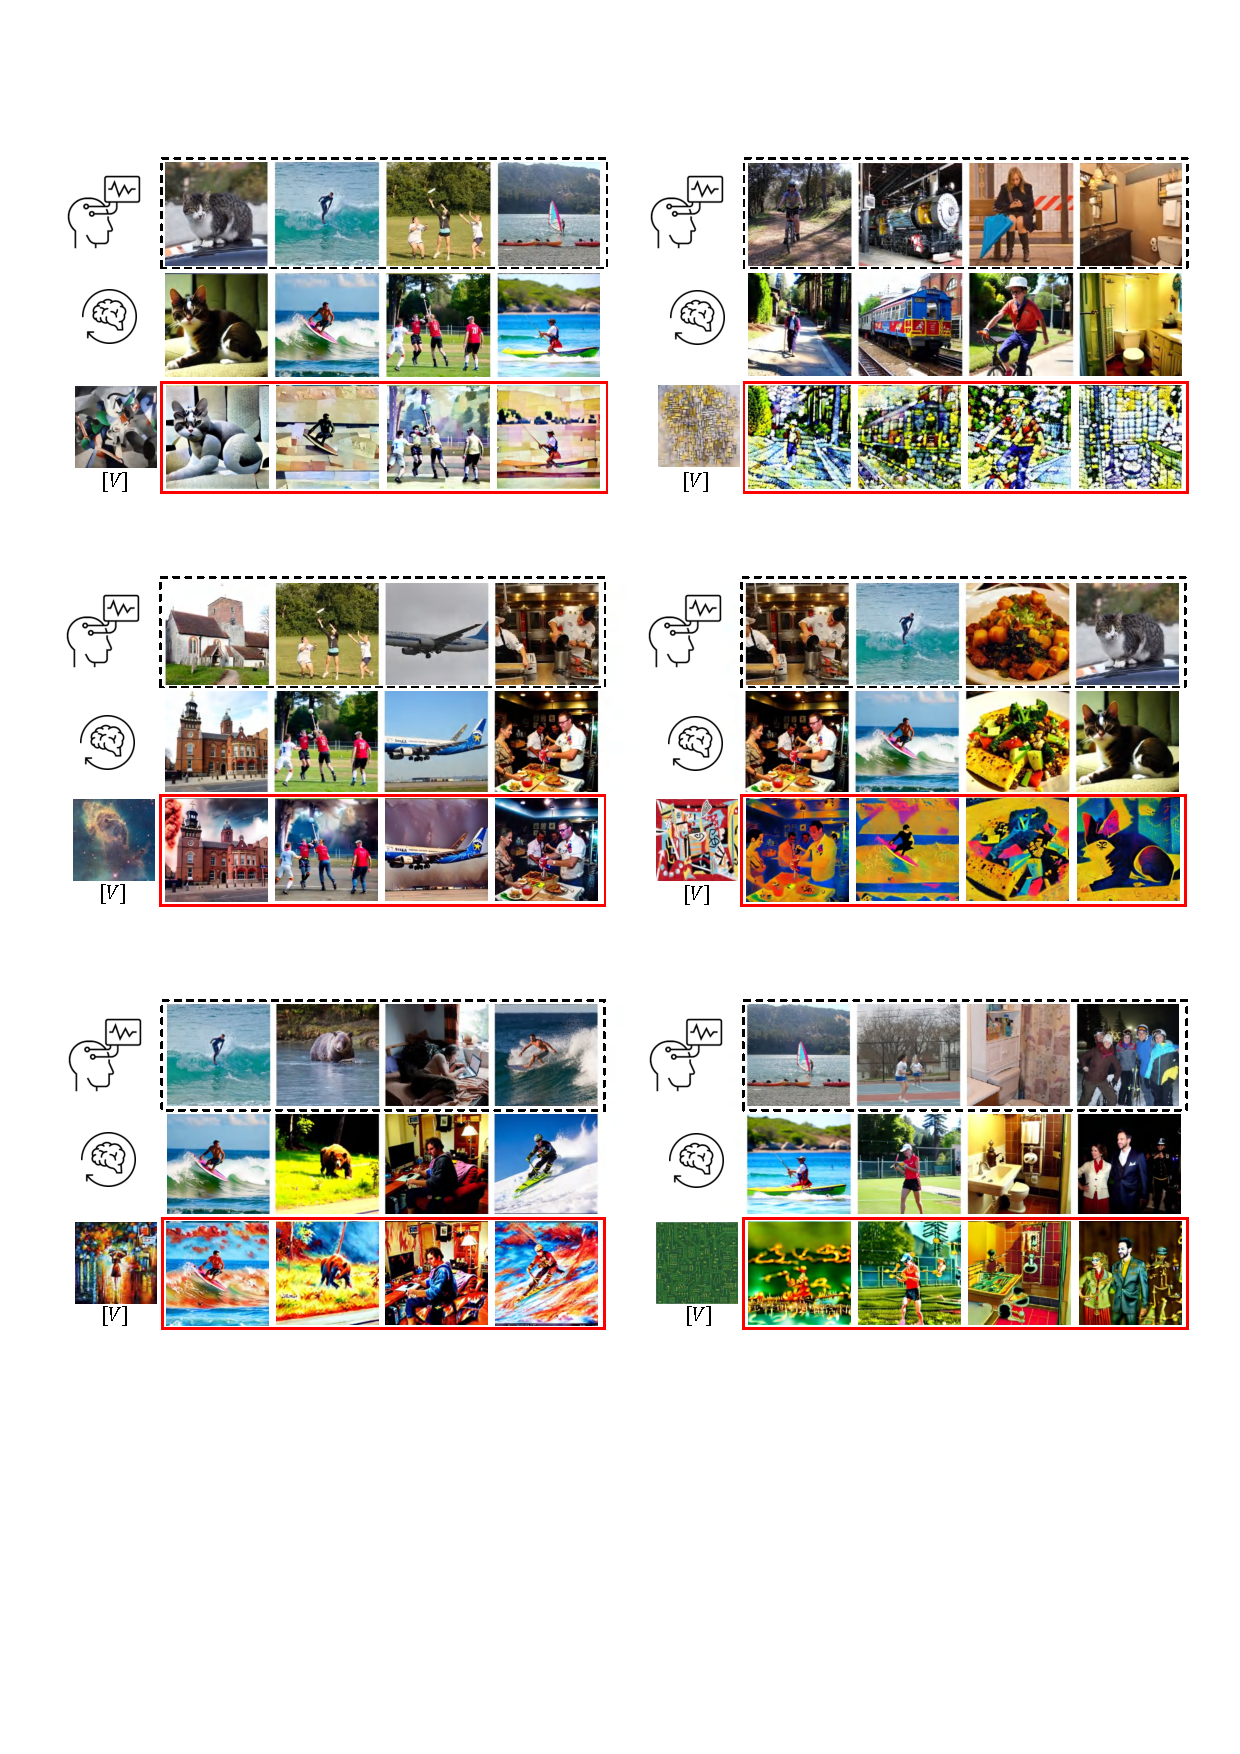
\includegraphics[width=1.0\textwidth]{figs/style_supp.pdf} 
    % \vspace{-4pt}
  \caption{\textbf{Demonstration Results of Multi-Modal Instruction.} First row list the visual stimulus while second row depict our intermediate reconstructions. The manipulation results via \emph{In the [V] style} are shown within red boxes of the last row.}
  \label{fig:supp_style}
  % \vspace{30pt}
\end{figure*}






% \begin{figure}[t!]
%   \centering
%   \includegraphics[width=0.98\textwidth]{figs/supp_results0.pdf} 
%     \vspace{-4pt}
%   \caption{\textbf{Image Manipulation Results by Visual Instruction.} }
%   \label{fig:supp_results0}
%   \vspace{-10pt}
% \end{figure}